\section{Methodologie de décolution du PO}%
\label{sec:methodologie_de_décolution_du_po}

\subsection{Introduction}

Bien que dans les chapitres précédents nous avons vu qu'il était possible d'estimer de
façon fiable la contribution des différentes sources de PM grâce aux PMF et d'établir une
phénoménologie des sources de \PMdix, la question de leur effet sanitaire n'est toujours
pas répondu. En effet, l'ordre de contribution à la concentration moyenne annuelle des
\PMdix{} présentée par \cite[(figure 3)]{weberComparison2019} ne préjugage pas de leurs
impacts sanitaires.

En effet, comme détaillé dans en introduction
section~\ref{sec:le_potentiel_oxydant_des_aerosols}, la mesure de la masse des PM n'est
certainement pas l'indicateur le plus adapté pour évaluer leur toxicité, car la composition
chimique, forme, surface réactive, etc. n'est pas prise en compte par cette métrique.
C'est pourquoi le potentiel oxydant (PO ou OP en anglais), mesurant indirectement les
espèces réactives de l'oxygène (ERO ou ROS en anglais) apportées ou induites par les PM,
est proposé comme nouvel indicateur de l'exposition des populations à la toxicité des PM. 
Il est maintenant bien documenté que les différents tests de PO présentent une information
différente de la concentration massique (voir par exemple,
\cite{choRedox2005,vermaReactive2014,batesReactive2015,fangOxidative2016,fangAmbient2017,calasSeasonal2019},
ou la revue détaillée récente de \cite{batesReview2019}), comme rappelé dans le
tableau~\ref{tab:calas_2018_spearman} sur une étude à Chamonix par
\cite{calasComparison2018} présentant la corrélation entre la masse des \PMdix{} et 5
mesures de PO.

Il est également connu que les différentes espèces chimiques constitutives des PM ne
réagissent pas à un même test de PO de la même manière. Notamment, les métaux de
transitions ainsi que certaines quinones conduisent à la formation d'un grand nombre de
\ce{HO^.} et sont donc des espèces très réactives à la mesure du PO
\autocite{charrierRates2015,calasImportance2017}.

\begin{table}[ht]
    \begin{ThreePartTable}
        \centering
        \caption{Corrélation de Spearman entre 5 tests de PO et la masse des \PMdix{} sur
            le site de Chamonix (2013) séparer en période chaude (triangle bas) et froide
            (triangle haut).\\
            Source : \cite[Table 3]{calasComparison2018}
        }
        \label{tab:calas_2018_spearman}
        \footnotesize
        \begin{tabular}{lSSSSSS}
            \toprule
             & {\PMdix} & {OP DTTv\tnote{1}} & {OP AAv\tnote{1}} & {OP ESRv\tnote{2}} & {OP GSHv\tnote{1}} & {OP ASCv\tnote{3}}\\
             \midrule
            \PMdix  &           & 0.91{***} & 0.91{***} & 0.59{***} & 0.87{***} & 0.90{***}\\
            OP DTTv & 0.71{***} &           & 0.89{***} & 0.61{***} & 0.79{***} & 0.72{***}\\
            OP AAv  & 0.43{*}   & 0.65{***} &           & 0.54{***} & 0.85{***} & 0.79{***}\\
            OP ESRv & 0.088     & 0.17      & 0.36      &           & 0.56{**}  & 0.59{**}\\
            OP GSHv & 0.44{*}   & 0.29      & 0.36      & 0.63{*}   &           & 0.92{***}\\
            OP ASCv & 0.38{*}   & 0.37{*}   & -0.072    & -0.29     & 0.17      & \\
            \bottomrule
        \end{tabular}
        \begin{tablenotes}
        \item[] *** p < 0.001 level, ** p < 0.01 level, * p < 0.05 level
        \item[1] n = 30 (cold period), n = 29 (warm period)
        \item[2] n = 30 (cold period), n = 14 (warm period)
        \item[3] n = 27 (cold period), n = 29 (warm period)
        \end{tablenotes}
    \end{ThreePartTable}
\end{table}

\subsubsection{Un PO par espèces chimiques ?}%
\label{sub:un_po_par_espèces_chimiques_}

Cependant, lorsque l'ensemble des PM est solubilisé, analysé et confronté aux PO, de
fortes corrélations sont bien observés avec les espèces présentant une forte réactivité aux
PO, mais certaines autres espèces sont parfois fortement corrélées alors qu'une mesure
directe de leurs PO montre aucune réactivité --c'est notamment le cas du nitrate,
de l'ammonium ou de lévoglucosan \autocite{vermaRedox2009,calasComparison2018,calasSeasonal2019}.

Ces corrélations ne reflètent donc pas de réelles causalité mais des co-corrélations. Le
lévoglucosan est émis en même temps que certaines quinones lors de la combustion de bois,
qui elles sont redox-active, et le nitrate est émis temporellement en fin d'hiver-début
printemps, où la combustion de biomasse est toujours présente. 
Ainsi, ces corrélations sont un premier pas vers l'identification des sources majoritaires
de PO, mais s'avère insuffisant.

\subsubsection{Du PO par espèces chimiques au PO par sources}

L'attribution d'un PO intrinsèque par espèces chimiques est donc estimée par mesure
directe ou par regression linéaire
multiple~\autocite{calasImportance2017,borlazaOxidative2018}. La première solution permet
la mesure exacte du PO de l'espèce mais présente des limitations analytiques évidentes
(composé pur, grand nombre d'espèces et de gamme de concentration à étudier), et la
deuxième peut présenter des ``faux positifs'' dans le cas où toutes les espèces chimiques
ne sont pas mesurées --ce qui est toujours le cas-- du fait de l'émission conjointe
d'espèce redox-active et non-redox-active (quinones et lévoglucosan par exemple).

Aussi, d'un point de vue réglementaire, il est souvent plus compréhensible d'agir sur
un secteur d'émission que sur une espèce chimique en particulier.

Pour ces raisons, l'agrégation de l'information géochimique par source d'émission plutôt
que par espèce chimique est intéressante :
\begin{enumerate}
    \item le nombre d'inconnues diminue drastiquement (plusieurs milliers d'espèces
        chimique à une dizaine de sources d'émission);
    \item pas besoin d'identifier chaque espèces chimiques du moment que les sources
        majoritaires sont bien représentées;
    \item la contribution des sources aux potentiels oxydants est davantage transmissible
        en termes de politiques publiques que la contribution d'espèces chimiques;
\end{enumerate}

Pour estimer un PO par sources, plusieurs méthodes sont possibles : 1) introduire le PO
comme variable dans une étude de source (CMB, PMF, etc.) 2) faire une étude de source
(CMB, PMF, etc.) grâce à l'information chimique et ensuite établir un modèle d'inversion
entre les sources identifiées et les PO.

\cite{vermaReactive2014} ont utilisé les 2 méthodes en introduisant le
\PODTT{} dans une PMF avec comme autres espèces WSOC\footnote{WSOC: Water soluble
organic carbon}, BrnC\footnote{BrnC: Brown Carbon}, EC, \SOq, \NHt, K, Ca, Mn, Fe, Cu et
Zn, mais également en établissant une régression linéaire entre le \PODTT{} et les sources
issues du CMB.
Entre 2014 et 2017, \cite{batesReactive2015} puis \cite{fangOxidative2016}, de la même
équipe de recherche, ont repris ce principe et l'ont appliqués à plus grande échelle
spatiale et également au \POAAv.

\begin{figure}[ht]
    \centering
    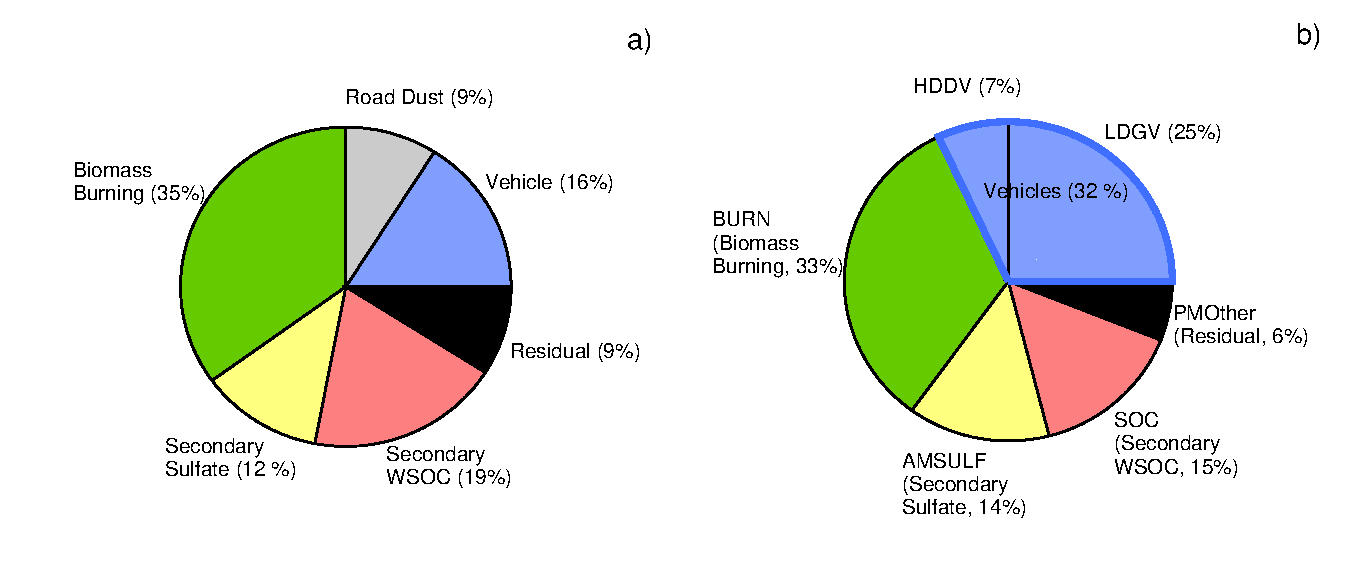
\includegraphics[width=1.0\linewidth]{figures/chapter04/verma_2014_fig8.pdf}
    \caption{Première estimation de la contribution des sources de PM au \PODTT{} par
        \cite[][figure 8]{vermaReactive2014}: \textbf{a)} par ajout du DTT dans la PMF et
        \textbf{b)} par régression linéaire entre \PODTT{} et CMB.
    }%
    \label{fig:figures/chapter04/verma_2014_fig8}
\end{figure}

Seulement, nous avons vu que les PMF sont très sensible aux variables utilisées. Or, leurs
études PMF inclut un ensemble d'espèce chimiques restreint (une dizaine de métaux et le
WSOC), en plus du PO. Seuls 4 facteurs sont identifiés par \cite{fangOxidative2016}, ce
qui semble peu au regard des PMF utilisant un jeu d'espèce chimique plus conséquente (voir
notamment tous le chapitre précédent). En plus, ce faible nombre d'espèces chimiques
associés à une nouvelle variable, le PO, dont nous ne connaissons a priori que peu de chose de ses
sources, peut conduire à des solutions instables statistiquement.

La solution utilisant la régression linéaire à partir du CMB hérite des limitations
propre au CMB : peu de prise en compte des particularités locales, connaissance a priori
forte, etc (voir section
~\ref{ssub:atouts_et_limitations_des_différents_modèles_récepteurs}).
Ainsi, \cite{batesSource2018} utilise un modèle CMB pour prédire à large échelle spatiale
(Amérique du Nord) le PO, mais le modèle établit présente de faible performance
statistique ($r^2 = 0.36$ et intercepte non nul), notamment du fait de l'oubli potentiel de
sources importantes (bioaérosols \autocite{samakeUnexpected2017}, etc).

\subsubsection{Couplage de PMF avancée avec l'estimation du PO}%
\label{sub:couplage_de_pmf_avancée_avec_l_estimation_du_po}

Je propose dans cette section de coupler les connaissances acquises sur les PMF présentées
dans le chapitre~\ref{cha:approfondissement_des_connaissances_des_sources_des_pm}
précédent, en n'ajoutant pas le PO comme variable explicative pour ne pas perturber le
modèle, puis d'évaluer le PO intrinsèque (i.e. par microgramme) de chacune des sources
identifiées, illustré par la figure~\ref{fig:workflow_inversion}.

Le site de Chamonix entre 2013 et 2014 a été choisi pour tester cette méthode du fait
d'une étude PMF approfondie par \cite{chevrierChauffage2016} et par les mesures de PO sur
ce site effectué lors de la thèse de \cite{calasPollution2017}, aussi bien pour le \POAA{}
que le \PODTT, et a fait l'objet d'une publication présenté ci-après.

\begin{figure}[ht]
    \centering
    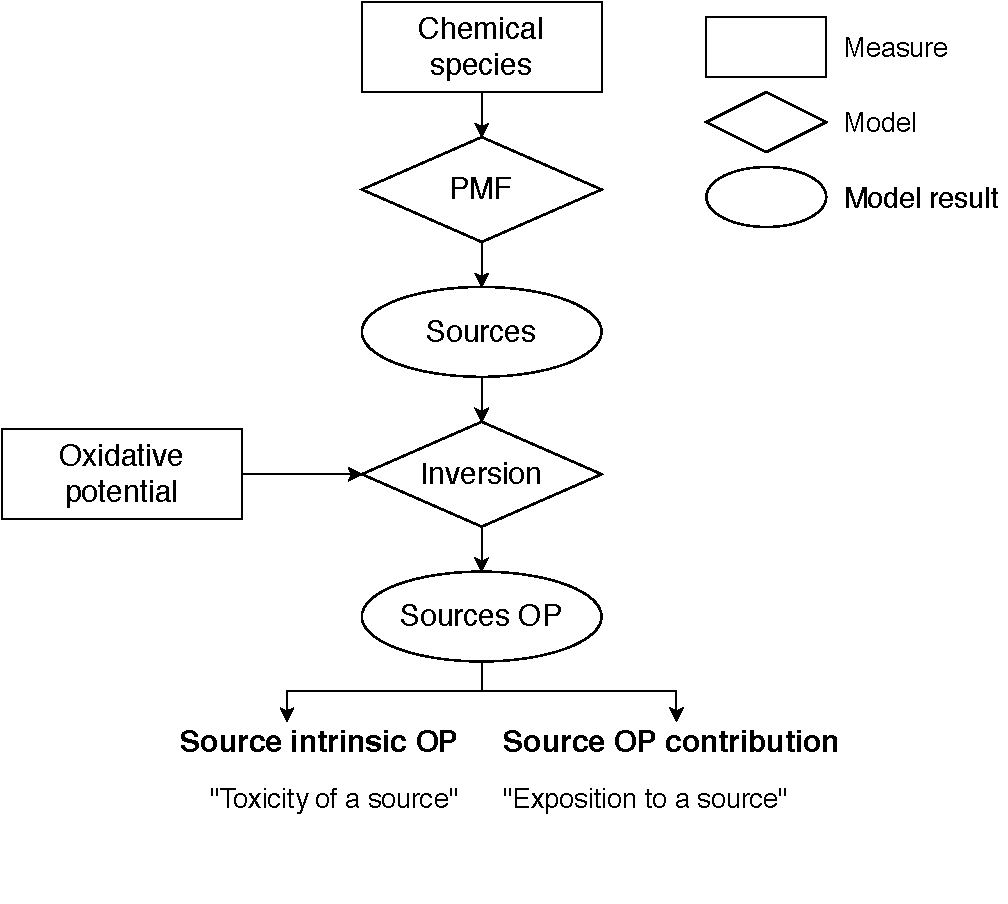
\includegraphics[width=0.8\linewidth]{figures/chapter04/flowchart_inversion.pdf}
    \caption{Processus suivi afin d'estimer la contribution des sources de PM aux
        potentiels oxydants. La méthode d'inversion utilisée dans ce chapitre est une
        régréssion linéaire multiple, permettant d'attribuer un PO par microgramme de source
        (\textit{PO intrinsèque}), estimant la ``toxicité de la source'', et la contribution de
    chacune des sources aux PO, estimant l'exposition de la population à cette source.}%
    \label{fig:workflow_inversion}
\end{figure}

\clearpage
\subsection{An apportionment method for the oxidative potential of atmospheric particulate
matter sources: application to a one-year study in Chamonix, France}
\label{sec:weber_et_al_2018}

Article paru dans le journal \textit{Atmospheric Chemistry and Physics} le 4 juin 2019 :

\begin{quote}
    Samuël Weber, Gaëlle Uzu, Aude Calas, Florie Chevrier, Jean-Luc Besombes,
    Aurélie Charron, Dalia Salameh, Irena Ježek, Griša Močnik, et Jean-Luc Jaffrezo. 2018.
    \textit{An Apportionment Method for the Oxidative Potential of Atmospheric Particulate
    Matter Sources: Application to a One-Year Study in Chamonix, France}. Atmospheric
    Chemistry and Physics 18(13), pp. 9617‑9629.
    \textsc{doi} : \href{https://doi.org/10.5194/acp-18-9617-2018}{10.5194/acp-18-9617-2018},
    \textsc{url} : \url{https://www.atmos-chem-phys.net/18/9617/2018/}
\end{quote}

Les profils PMF, la corrélation entre espèces chimiques et PO et sources et
PO à titre de comparaison avec les études antérieures, sont présentés en complément de
l'article, repris en annexe~\ref{annexe:deconvol_OP_SI}.

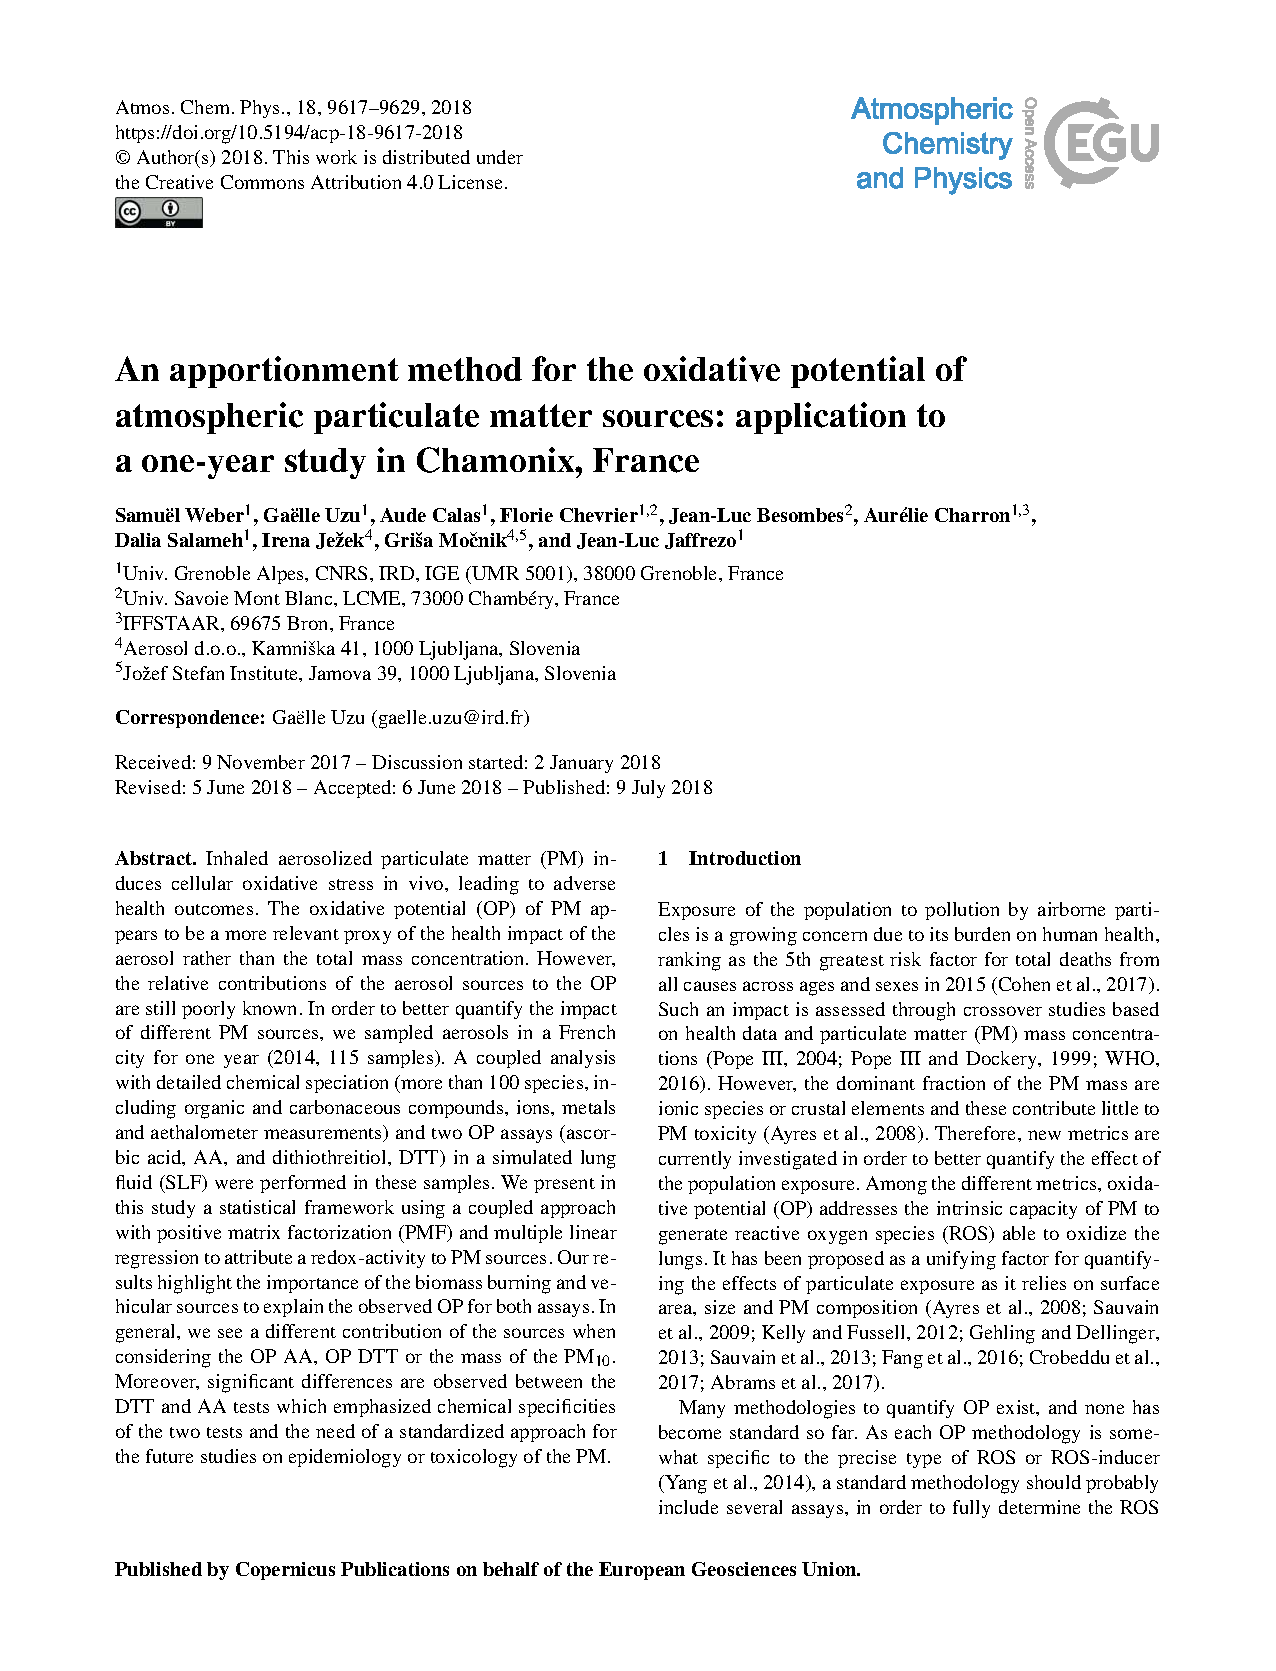
\includepdf[pages=-,scale=0.95,pagecommand={\pagestyle{fancy}}]{chapters/deconvol_OP.pdf}


\subsection{Conclusion}

Ce chapitre prouve tout d'abord qu'il est possible de déterminer les sources de PO grâce à
une étude couplée entre une PMF avancée utilisant différents traceurs organiques résultant
en 8 facteurs distincts et une régression linéaire multiple prenant en compte
la mesure du PO à iso-masse utilisant des conditions de bioaccessibilité proche du milieu
pulmonaire et ses incertitudes, avec une très bonne performance statistique.

Cette méthode permet de différencier très nettement les sources de PM contribuant aux PO
et apporte une vue nouvelle de l'aérosol en redistribuant l'importance de la contribution
des sources. Conformément aux résultats des 3 études précédentes faites aux États-Unis
\autocite{vermaReactive2014,batesReactive2015,fangOxidative2016}, la combustion de
biomasse domestique et le transport routier représentent les 2 sources principales de
\POAAv{} et \PODTTv.

L'utilisation de deux tests de PO nous permet aussi d'affirmer que ces 2 tests ne portent
pas en eux exactement les mêmes informations géochimiques, car les sources de PM les
expliquant diffèrent --bien que la même tendance générale est observée. En l'absence
d'étude approfondie quant aux liens toxicologie-PO ou épidémiologie-PO, le maintient de
différents tests de PO est donc recommandé.

Aussi, certaines corrélations observées, aussi bien avec des espèces chimiques que des
facteurs PMF, s'avère comme attendue trompeuse. Le facteur nitrate-rich était corrélé au
\POAAv{} mais présent en réalité un PO intrinsèque quasi-nul. Inversement, le facteur
secondaire biogénique, tracé par le MSA, est négativement corrélé aux deux \OPv{} alors
qu'il présente le 2\ieme{} \PODTT{} intrinsèque le plus élevé. Il est donc nécessaire
d'utiliser des méthodes statistiques plus avancées que la régression uni-variée lorsque
l'on cherche à estimer les sources de PO afin de s'affranchir des tendances sainonières et
des covariations entre espèces.

Cette méthode est donc validée comme outil de déconvolution des sources de PO, et le
prochain chapitre traitera de son application à un large panel d'environnement et année
d'étude, afin d'établir à la manière du chapitre précédent, une phénoménologie non pas des
sources de la masse \PMdix, mais des sources de PO.


\section{Synthèse grande échelle}%
\label{sec:synthèse_grande_échelle}

\subsection{Article}%
\label{sub:article}

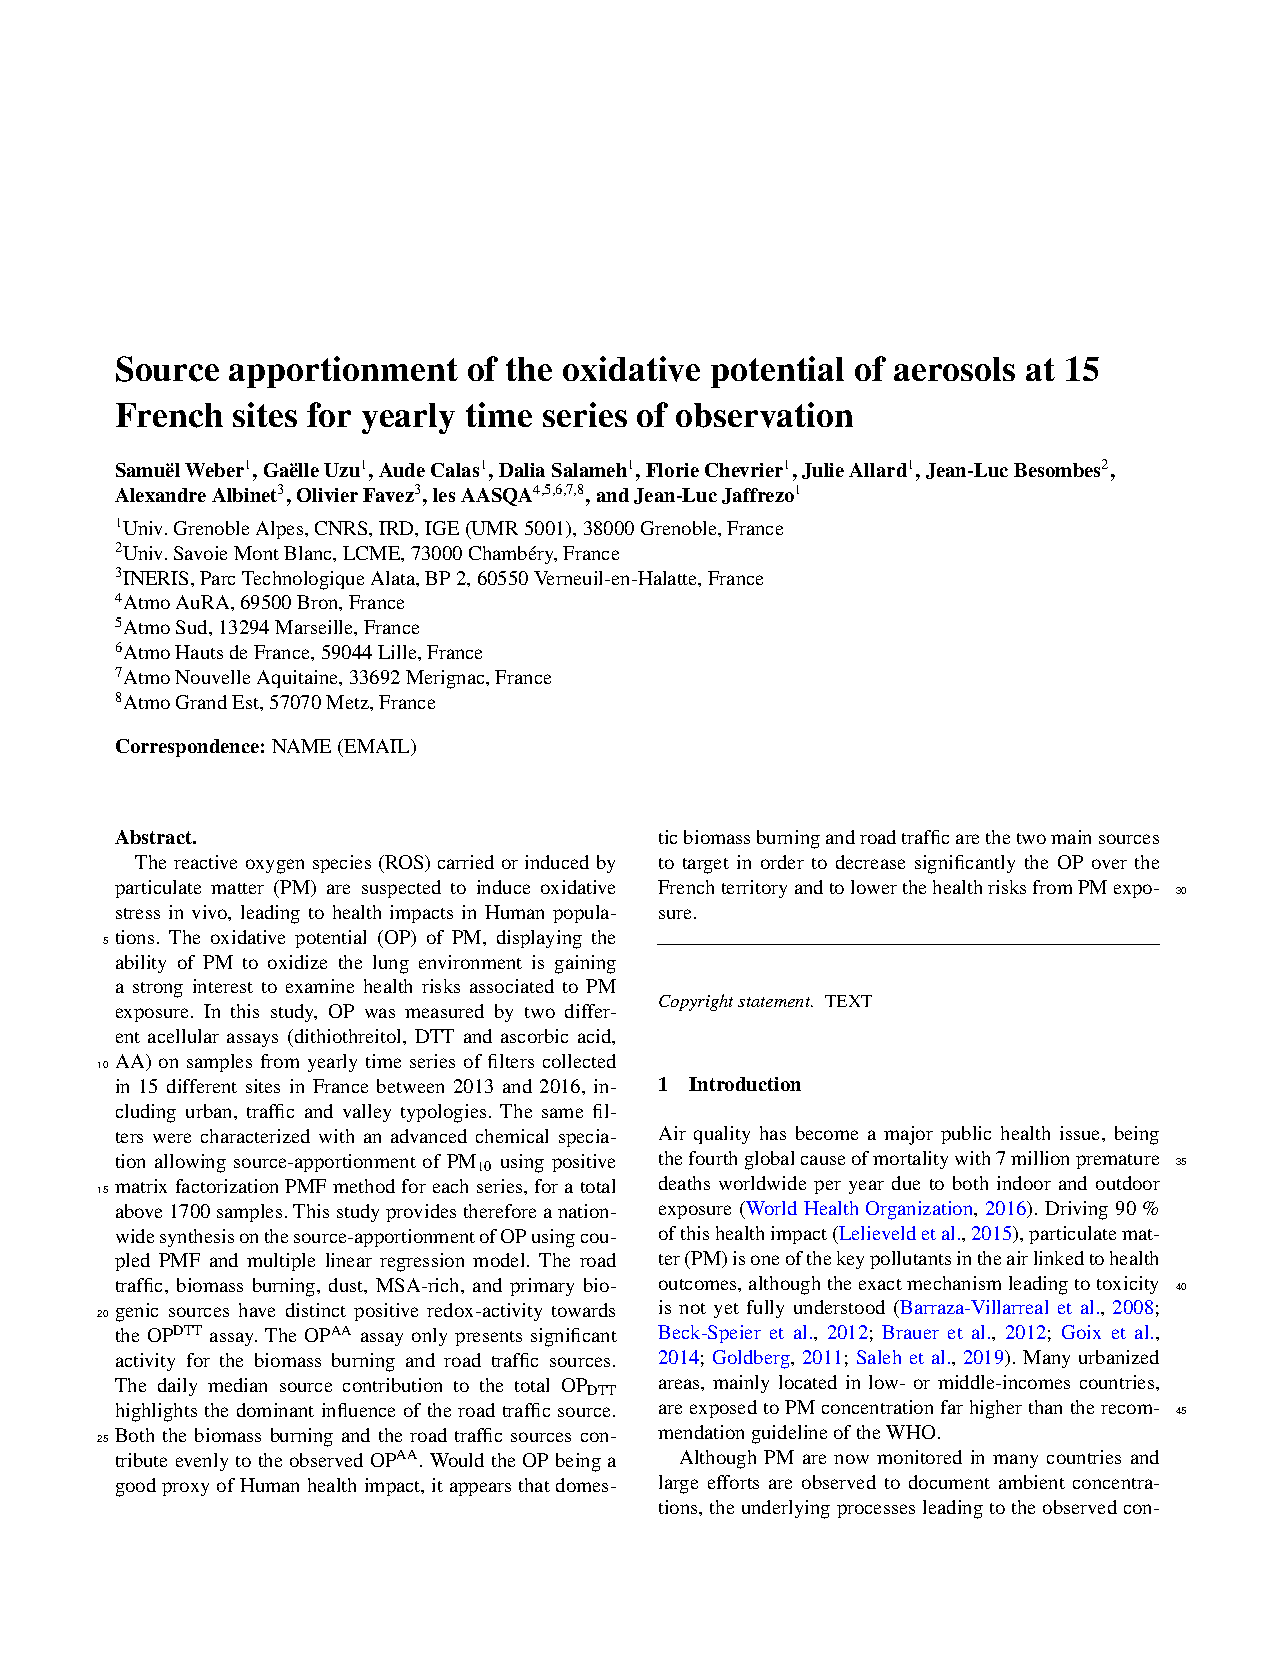
\includepdf[pages=-,scale=0.95,pagecommand={\pagestyle{fancy}}]{chapters/article_allOP/article_nuage.pdf}
